\documentclass[10pt,twocolumn,letterpaper]{article}

% Pacotes basicos - maxima compatibilidade Windows
\usepackage{geometry}
\usepackage{times}
\usepackage{titlesec}
\usepackage{url}
\usepackage{graphicx,xcolor,comment,enumerate,multirow,multicol} 
\usepackage{amsmath,amsthm,amsfonts,amssymb,dsfont,mathtools, array}

\usepackage{enumitem}
\setlist[itemize]{
    itemsep=2pt,        % Espaçamento vertical entre itens
    parsep=0pt,         % Espaçamento entre parágrafos dentro de um item
    topsep=0pt,         % Espaçamento vertical antes do primeiro item da lista
    partopsep=0pt,      % Espaçamento extra quando a lista começa no início de um parágrafo
    leftmargin=1.5em    % Opcional: Ajusta a margem esquerda (se estiver muito indentado)
}

% Configuracao da pagina
\geometry{
    letterpaper,
    left=0.75in,
    right=0.75in,
    top=0.75in,
    bottom=1in
}

%% Edição confortável
% Inclui o pacote xcolor com a opção para nomes de cores
\usepackage[svgnames]{xcolor}
% Para desativar comente a linha utiliando %
%% Define a cor do texto usando o código hexadecimal
\definecolor{Cornsilk}{HTML}{FFF8DC}

% Define a cor de fundo da página como preta
\pagecolor{Black}

% Define a cor padrão do texto para todo o documento
\color{white}

% Configuracao das secoes
\titleformat{\section}[block]
{\normalfont\fontsize{10}{12}\bfseries}
{\thesection.}{0.5em}{}

% Remove numeracao das paginas
\pagestyle{empty}

% Configuracoes de espacamento
\setlength{\columnsep}{0.25in}
\setlength{\parindent}{0pt}
\setlength{\parskip}{6pt}

\begin{document}

% Titulo centralizado em coluna unica
\twocolumn[
\begin{center}
    {\fontsize{16}{19}\selectfont\bfseries 
    Experimento 3\\ Estudo dirigido sobre estruturas cristalinas}

    \vspace{1cm}
    
    {\fontsize{11}{13}\selectfont 
     Carlos E. da S. Papa – 232013390, Robson Lima De Oliveira – 211067362, Ronan Cunha Freitas – 232013425 }

    \vspace{0.35cm}   

    {\fontsize{11}{13}\selectfont 
    Turma 01}
    
    \vspace{1cm}  
\end{center}
]

\section{OBJETIVOS}

\hspace{1cm} Os objetivos são: estudo do efeito fotoelétrico, determinação da constante de Planck, determinação da função trabalho da fotocélula e determinação da frequência de corte para a fotocélula. 

% \vspace{.75cm}

\section{MATERIAIS e EQUIPAMENTO UTILIZADOS}

\begin{itemize}
    \item Fotocélula;
    \item Rede de difração, 600 linhas/mm;
    \item Filtros, 580 nm e 525 nm;
    \item Fenda de abertura ajustável;
    \item Lente convergente, f + 100 nm;
    \item Lãmpada de mercúrio;
    \item Trilho de sustentação;
    \item Amplificador universal de medição;
    \item Multímetro digital.
\end{itemize}

% \vspace{.75cm}

\section{PROCEDIMENTOS EXPERIMENTAIS}

\hspace{1cm} Faça-se a montagem do experimento como indicado na figura (1) com a lãmpada de mercúrio e a fotocélula nas extremidades do trilho. E então posiciona-se a fenda ajustável a aproximadamente 9 cm da lãmpada, e a lente a 20cm da mesma. 

\begin{figure}[h]
    \centering
    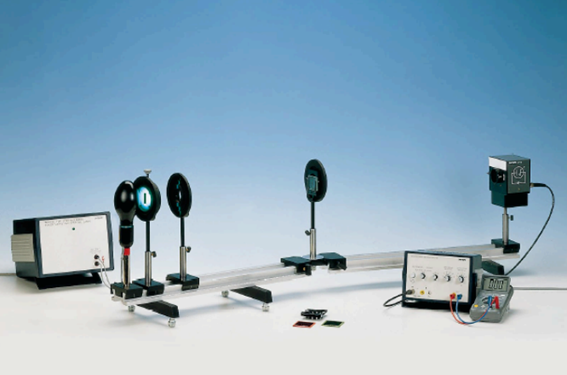
\includegraphics[width=7cm]{Imagem1.png}
    \caption{Montagem do experimento}
    \label{fig:label}
\end{figure}

\hspace{1cm} Posteriormente, liga-se a lãmpada e focalizando o feixe de luz na fotocélula, movimentando-se o suporte da lente sobre o trilho. Certifica-se que a janela da fotocélula esteja fechada. Então, ajusta-se a abertura da fenda para que a imagem formada na fotocélula tenha a largura a cerca de 1 cm. 

\noindent Antes de conectar a fotocélula ao amplificador deve-se:

\begin{itemize}
    \item Amplificador
    \begin{itemize}
        \item Modo de operação: eletrômetro $(R_e > 10^{13} \, \Omega)$.
        \item Amplificação: 100.
        \item Constante de tempo: 0.
    \end{itemize}
    \item Voltímetro
    \begin{itemize}
        \item Escala 2V DC.
    \end{itemize}
\end{itemize}

\vspace{.25cm}

\hspace{1cm} Em seguida, ajusta-se o zero do amplificador atuando-se no botão ”0” mantendo o botão de descarga da fotocélula pressionado, acompanhando o valor da saída com o voltímetro. E por fim, para realizar a medição segue-se os seguintes passos: 

\begin{itemize}
    \item Movimente o trilho para selecionar a faixa monocromática desejada. \item Com a janela da fotocélula fechada, verifique o zero do amplificador. 
    \item Abra a janela e espere alguns segundos para o valor de tensão no voltímetro se estabilizar e faça a leitura. 
    \item Feche a janela da fotocélula. 
\end{itemize}

\hspace{1cm} Durante todo o processo deve-se lembrar das seguintes
observações:

\begin{itemize}
    \item Liga-se os equipamentos 15 minutos antes de fazer as medidas. 
    \item Evite desligar a lãmpada, pois uma vez desligada, só será possível religa-la após seu resfriamento. O que leva aproximadamente 10 minutos. 
    \item Não toque na lãmpada, a temperatura do bulbo pode ultrapassar 100ºC. 
    \item Nunca olhe diretamente para a abertura da lãmpada, a radiação ultravioleta é nociva a sua visão. 
    \item Só abra a janela da fotocélula durante as medições. Fora desta condição a janela deve ficar sempre fechada. 
\end{itemize}

% \vspace{.75cm}

\section{RESULTADOS EXPERIMENTAIS}
\hspace{1cm} Seguindo o procedimento experimental obtemos os seguintes resultados no laboratório:

\vspace{-.25cm}

\begin{table}[htbp]
    \centering
    \caption{Medições de Tensão em Função da Corrente DC}
    \label{tab:medicoes_tensao}
    \vspace{0.25cm}
    \begin{tabular}{ccc}
        \hline
        \rule{0pt}{3ex}\textbf{Faixa Monocromática} & \textbf{Ângulo} [°] & \textbf{Tensão} [V]\\[5pt]
        \hline
        \rule{0pt}{3ex}Azul 1 & 12 & 0.65 \\
        Azul 2 & 14 & 0.52 \\
        Azul 3 & 16 & 0.51 \\
        Verde & 20 & 0.32 \\
        Laranja & 21 & 0.20 \\[5pt]
        \hline
    \end{tabular}
\end{table}

\vspace{-.25cm}

\noindent Partindo do Princípio de Huygens temos a seguinte relação:

\vspace{-.5cm}

\begin{equation*}
    n\,\lambda = d\, \sin{\theta}
\end{equation*}

\vspace{-.15cm}

\hspace{1cm} Em que $\lambda$ é o comprimento da onda eletromagnética no vácuo e d a distãncia entre as linhas da rede de difração:

\vspace{-.5cm}

\begin{equation*}
    \lambda = \frac{c}{v}
\end{equation*}

\vspace{-.4cm}

\begin{equation*}
    d = \frac{1}{600}\cdot10^{-3}\,\,[m] = 1.667 \cdot 10^{-6} \,\, [m]
\end{equation*}

\vspace{-.1cm}

\hspace{1cm} Durante este experimento tomamos os dados do primeiro harmônico. Assim, utilizamos a seguinte relação para obter as frequências de cada faixa:

\vspace{-.25cm}

\begin{equation*}
    v = \frac{c}{d\,\sin{\theta}}, \quad c = 299'792'458 \,\, \left[\frac{m}{s}\right]
\end{equation*}

\noindent E assim preenchemos a seguinte tabela:

\begin{table}[htbp]
    \centering
    \caption{Medições de Tensão em Função da Corrente DC}
    \label{tab:medicoes_tensao}
    \vspace{0.25cm}
    \begin{tabular}{ccc}
        \hline
        \rule{0pt}{3ex}\textbf{Faixa} & \textbf{Frequência} [Hz] & \textbf{Tensão} [V]\\[5pt]
        \hline
        \rule{0pt}{3ex}Azul 1 & $8.651532\cdot 10^{14}$ & 0.65 \\
        Azul 2 & $7.435271\cdot 10^{14}$ & 0.52 \\
        Azul 3 & $6.525802\cdot 10^{14}$ & 0.51 \\
        Verde & $5.259207\cdot 10^{14}$ & 0.32 \\
        Laranja & $5.019296\cdot 10^{14}$ & 0.20 \\[5pt]
        \hline
    \end{tabular}
\end{table}

\hspace{1cm}  Foi realizada a regressão linear, como mostra a seguinte figura:

\begin{figure}[h]
    \centering
    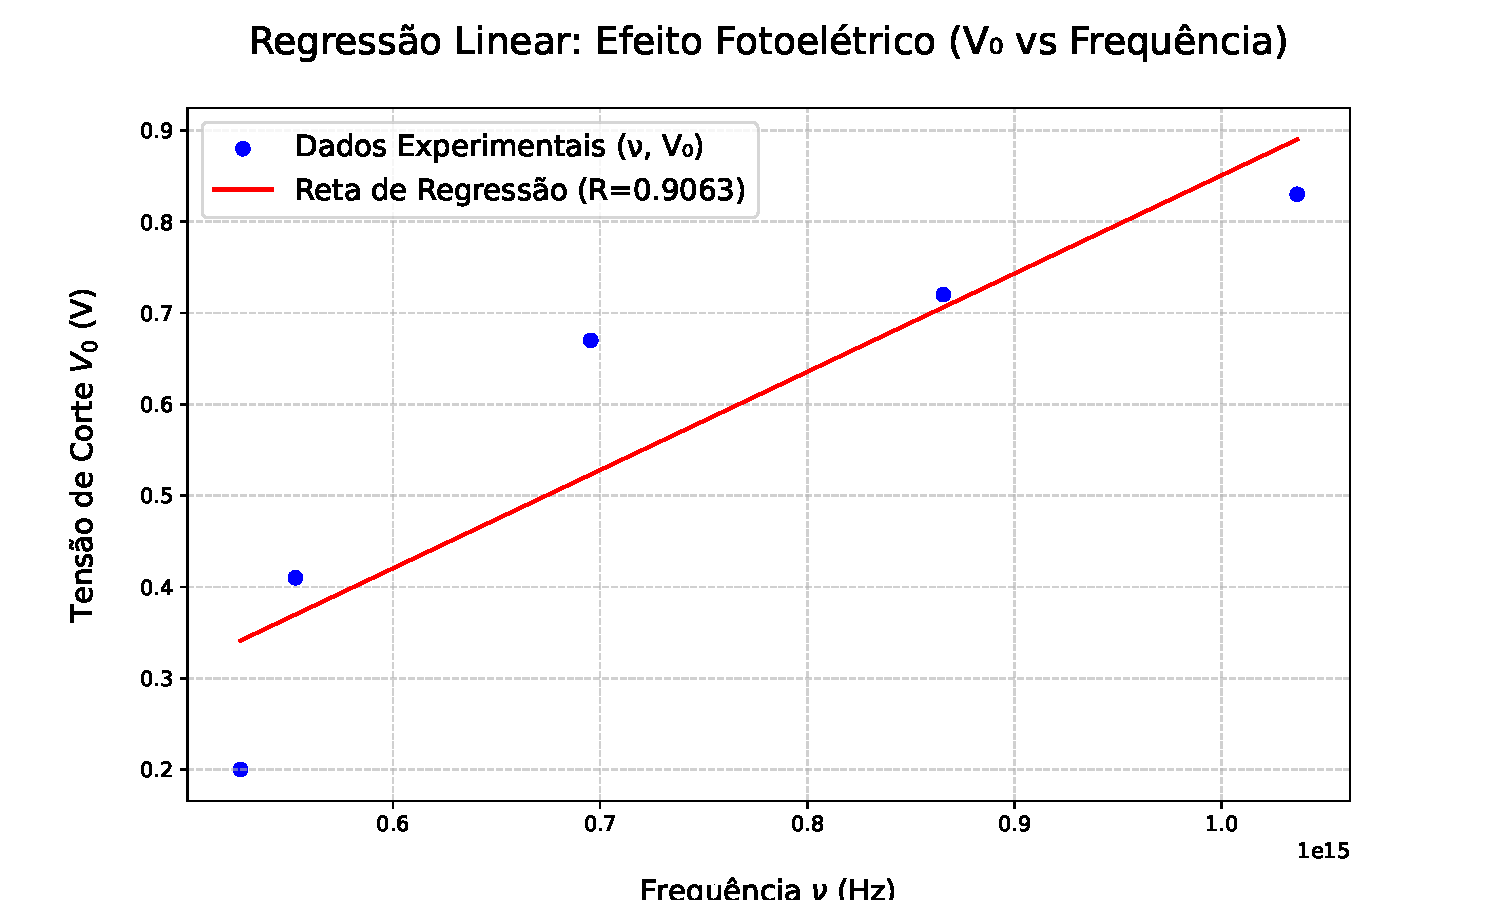
\includegraphics[width=8.5cm]{efeito_fotoeletrico_regressao.pdf}
    \caption{Resultados distribuidos graficamente}
    \label{fig:label}
\end{figure}

\noindent Assim obtivemos a seguinte equação:

{\Huge \color{red} *VER* EQUAÇÕES}

{\color{red} Não sei da onde veio esses valores e essas equações.}

\begin{equation*}
    V_0 = 8.651532\cdot 10^{14} \cdot v - 4.76700997e-20
\end{equation*}

\hspace{1cm} Dividindo a equação acima pela carga do elétron $(e =
1.6 \cdot 10^{-19} \,\, [C])$, temos:

\begin{equation*}
    K_{\max} = eV_0 = 1.7211 \cdot 10^{-34}\,v - 0.225054003\,e
\end{equation*}

\hspace{1cm} Sabendo que $K_{\max} = h\,v - \Phi\,$, obtemos a constante de
Planck e a função trabalho:

\begin{equation*}
    h = 1.7211\cdot 10^{-34} \,\, [J\,.\,s]
\end{equation*}

\begin{equation*}
    \Phi = 0.225054003\,e
\end{equation*}

\noindent Por fim, a frequência de corte é obtida quando $K_{\max} = 0$:

\begin{equation*}
    v_0 = 2.09218 \cdot 10^{14} \,\, Hz
\end{equation*}

% \vspace{.75cm}

\section{ANALISE DOS RESULTADOS EXPERIMENTAIS}

\noindent\textit{A. Sobre o valor da constante de Planck e potencial de
retardo}

\noindent O valor teórico da constante de Planck é em torno de:

\begin{equation*}
    h = 6.63 \cdot 10^{-34} \,\, [J\,.\,s]
\end{equation*}

\hspace{1cm} Ao comparar esse valor com o resultado obtido experismentalmente percebemos uma pequena perda devido a sensibilidade da fotocélula, além da impossibilidade de limitar a entrada de luz em uma única frequência. Mesmo assim, o valor permanece na mesma ordem de grandeza do esperado.

\hspace{1cm} Além disso, pelos cálculos da seção anterior vemos que materiais de potencial de retardo maiores gerariam valores maiores da constante de Planck, ou seja, utilizando-se lãmpadas de materiais com potenciais de retardo maior geraria um resultado mais preciso.

\noindent\textit{B. Sobre a função trabalho e frequência de corte}

\hspace{1cm} A função trabalho é a energia mínima necessária para que um elétron se desprenda de um material. Portanto, podemos utilizar a função trabalho para caracterizar o material da fotocélula.

\hspace{1cm} A frequência de corte está relacionada a função trabalho do material e é a frequência mínima necessária para que a energia do fóton absorvido pelo elétron seja o suficiente para que o mesmo seja emitido do material.

\hspace{1cm} Não conseguimos explicar o efeito fotoelétrico utilizando apenas a física clássica pois a teoria clássica não abrange a dualidade onda-particula do elétron.

\noindent\textit{C. Sobre a célula fotoelétrica e a relação de absorção de
fótons na frequência de corte e a tensão medida.}

\hspace{1cm} A Luz que passa através de uma janela de quartzo cai sobre uma placa de metal e libera elétrons, chamados de fotoelétrons. Esses elétrons podem ser detectados na forma de corrente se forem atraídos para o coletor metálico, por conta de uma diferença de potencial entre a placa metálica e o coletor metálico. . Se a tensão V aplicada é muito grande, a corrente fotoelétrica atinge um valor limite no qual todos os fotoelétrons emitidos pela placa de metal são coletados pelo coletor.

\hspace{1cm} A frequência de corte é o limiar onde o efeito fotoelétrico deixa de ocorrer para frenquêcias menores que ela. Se houver luz sobre o catodo, e a frenquência dela for maior que a de corte, haverá pelo menos um fóton que o atinge, e esse fóton será imediatamente absorvido por algum átomo causando a emissão imediata de um fotoelétron.

% \vspace{.75cm}

\section{Conclusão}

\hspace{1cm} Durante o experimento, foi possível observar o efeito fotoelétrico com o auxílio dos conceitos da física quãntica.

\hspace{1cm} Por meio desse experimento foi visto que a energia da emissão do elétron da fotocélula esta associada diretamente com a frenquência e não com a intensidade da luz emitida no material. Por meio dessa relação entre a frequência e o efeito fotoelétrico, foi possível encontrar a frequência de corte da célula fotoelétrica.

\hspace{1cm} As características observadas durante o experimento só foram possíveis de se explicar, levando em conta a dualidade do comportamento da luz, que se propaga como onda e interage com a matéria como partícula.

% \vfil
\section{REFERENCIAS BIBLIOGRAFICAS}

{\small
\begin{enumerate}

    \item CESCHIN, Artemis M. Apostila de materiais eletricos e magneticos.

    \item REZENDE, Sergio M. Materiais e Dispositivos Eletrônicos. 2ª ed. São Paulo: Editora Livraria da Física, 2004.

    \item HAYT, W. H. Jr. Eletromagnetismo. 6ª ed. Rio de Janeiro: LTC, 1995.
    
\end{enumerate}
}

\end{document}